\documentclass[10pt]{article}
\usepackage{titling} % Customize the title
\usepackage[utf8]{inputenc}
\usepackage{eso-pic}
\usepackage{charter}
\usepackage[margin=1in]{geometry}
\usepackage{amssymb,pdfpages,fancyhdr,subcaption,graphicx,hyperref,float,outlines,amsmath,gensymb}
\usepackage{listings}
\usepackage{parskip}
\usepackage{multicol} % Added the multicol package
\usepackage{booktabs}
\usepackage{graphicx}
\usepackage{subcaption}
\usepackage[style=numeric]{biblatex}
\usepackage{lipsum}
\addbibresource{refs.bib}

\usepackage{multirow}
\usepackage{listings}
\usepackage{xcolor}

% Define colors for code highlighting
\definecolor{codegreen}{rgb}{0,0.6,0}
\definecolor{codegray}{rgb}{0.5,0.5,0.5}
\definecolor{codepurple}{rgb}{0.58,0,0.82}
\definecolor{backcolour}{rgb}{0.95,0.95,0.92}

% Define settings for Python code
\lstdefinestyle{mystyle}{
    backgroundcolor=\color{backcolour},
    commentstyle=\color{codegreen},
    keywordstyle=\color{blue},
    numberstyle=\tiny\color{codegray},
    stringstyle=\color{codepurple},
    basicstyle=\ttfamily\footnotesize,
    breakatwhitespace=false,
    breaklines=true,
    captionpos=b,
    keepspaces=true,
    numbers=left,
    numbersep=5pt,
    showspaces=false,
    showstringspaces=false,
    showtabs=false,
    tabsize=2
}

\lstset{style=mystyle}

\title{\vspace{-3cm}\textbf{4M17 Coursework \#2 - Optimisation Algorithm Performance Comparison}}
\author{\vspace{-3cm}\textbf{Candidate No: 5730E}}

\begin{document}
\maketitle
\section{Abstract}
This report conducts a comparative analysis of two optimisation algorithms applied to minimise Keane's Bump Function, (KBF). In particular, the study focuses on a Continuous Genetic Algorithm, (GA), as well as an alternative algorithm not covered in the lectures: the State Transition Algorithm, (STA).

\begin{multicols}{2}

\section{Introduction}
\subsection{Keane's Bump Function}
\begin{figure}[H]
    \centering
    \begin{subfigure}{0.49\textwidth}
        \centering
        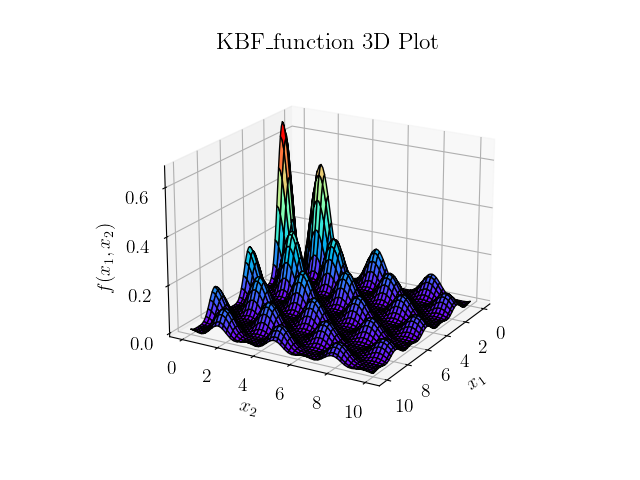
\includegraphics[width=\textwidth]{../figures/KBF_function_surf.png}
        \caption{Surface plot.}
        \label{fig:KBF_surf}
    \end{subfigure}
    \begin{subfigure}{0.49\textwidth}
        \centering
        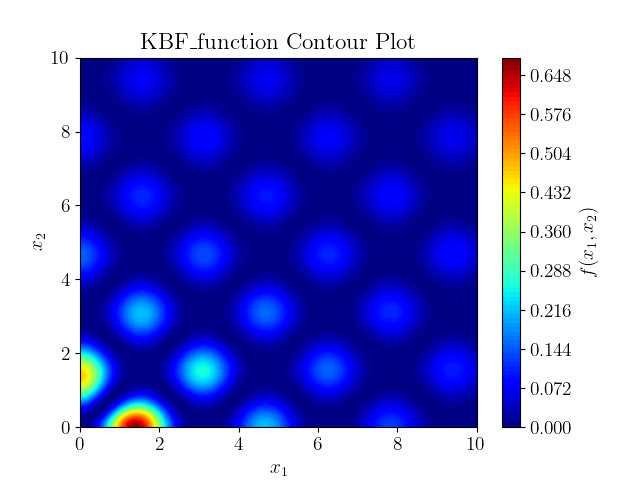
\includegraphics[width=\textwidth]{../figures/KBF_function_contour.png}
        \caption{Contour plot.}
        \label{fig:KBF_contour}
    \end{subfigure}
    \captionsetup{justification=centering}
    \caption{The two-dimensional visualisation of the Keane's Bump Function, (KBF).}
    \label{fig:KBF_2D}
\end{figure}
To compare the performances of the two algorithms, the Keane's Bump Function, (KBF), is used as the objective function. In particular, the n-dimensional constrained optimisation problem is defined as the maximisation of:

\begin{equation}
    f(\mathbf{x}) = \left| \frac{\sum_{i=1}^{n} (\cos(x_i))^4 - 2\prod_{i=1}^{n} (\cos(x_i))^2}{\sqrt{\sum_{i=1}^{n} i \cdot x_i^2}} \right| \\\vspace{1cm}
    \label{eq:KBF_cost}
\end{equation}
\begin{equation}
    \begin{aligned}
        \text{subject to} \quad & 0 \leq x_i \leq 10 \quad \forall i \in \{1, \dots, n\} \\
        & \quad \prod_{i=1}^{n} x_i > 0.75 \\
        & \quad \sum_{i=1}^{n} x_i < \frac{15n}{2}
    \end{aligned} 
    \label{eq:KBF_constraints}
\end{equation}

The two-dimensional form of the function has been plotted in Figure \ref{fig:KBF_2D}. Some notable properties are as follows:

\begin{itemize}
    \item The function is undefined at the origin, (0, 0). This is due to the division by zero in the denominator of Equation \ref{eq:KBF_cost}. Otherwise, the function is continuous and differentiable everywhere.
    \item The function is highly multi-modal. Its global maximum is located at the constaint boundary $x_{n}=0$, where $x_n$ denotes the final variable in the n-dimensional space. However, there are many local maxima located inside the feasible region.
    \item The function is nearly symmetric about the line $x_1=x_2$. This stems from its construction in \ref{eq:KBF_cost}, which primarily involves the the squares of individual input variables, $x_i^2$. This results some invariance reagrding the order of the input variables.
\end{itemize}
\end{multicols}

\section{Methodology}
\section{Results}
\section{Discussion}
\section{Conclusion}
\end{document}